% ===== UNIT 28: Post-processing contribution + input resolution (5.8-5.9) =====
% Status: REWRITTEN  (change to REWRITTEN / REVIEWED when done; see CHECKLIST.md)
% Rules: style rewrite only. Keep every \cite, \ref, \label, number, equation and table value as is. Change the wording, not the content.
\subsection{Post-processing contribution analysis}
Figure~\ref{fig:perstream} shows how much each post-processing step adds for each stream. Both streams start at a similar base performance ($\approx$82\% mAP). CLIP-SENet gains more from AQE ($+6.87$\,pp vs.\ $+1.86$\,pp for ViT-B). This is because the ResNet-IBN feature space has broader nearest-neighbour clusters, which benefit more from graph-based smoothing. The exact values are in the cumulative block of Table~\ref{tab:ablation}.

\begin{figure}[!t]
  \centering
  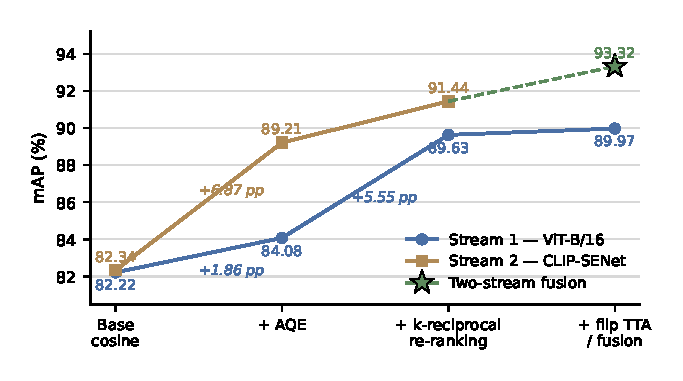
\includegraphics[width=0.92\columnwidth]{Fig8}
  \caption{Per-stream post-processing contribution on VeRi-776. The two streams
  start from almost identical base cosine accuracy but respond very differently
  to query expansion, and the fusion adds a further 1.88\,pp over the stronger
  post-processed stream}
  \label{fig:perstream}
\end{figure}

\subsection{Input-resolution sensitivity}
\label{sec:res_sens}
Stream~1 trains and evaluates at 224\,$\times$\,224. TransReID uses 256\,$\times$\,256 and CLIP-SENet uses 320\,$\times$\,320. This raises the question of whether the ViT-B stream loses accuracy at its lower resolution. We measure the inference-resolution sensitivity of the deployed checkpoint. We re-extract Stream~1 features at 256\,$\times$\,256 and 320\,$\times$\,320 (position embeddings are bicubically interpolated to the larger patch grid) and re-run the identical post-processing (Figure~\ref{fig:resolution}). Accuracy drops steadily away from the native resolution. The full-pipeline mAP drops by $0.30$\,pp at 256 and by $1.70$\,pp at 320. So the checkpoint is well matched to its training resolution, and higher-resolution inference does not help. Whether higher-resolution training would help (as in the 256 recipe of TransReID) is still open. It would require retraining (Section~\ref{sec:limitations}). The native-resolution result is also a further independent reproduction. This fresh extraction reproduces the headline 89.97\%\,/\,97.79\% operating point to within 0.03\,pp.

\begin{figure}[!t]
  \centering
  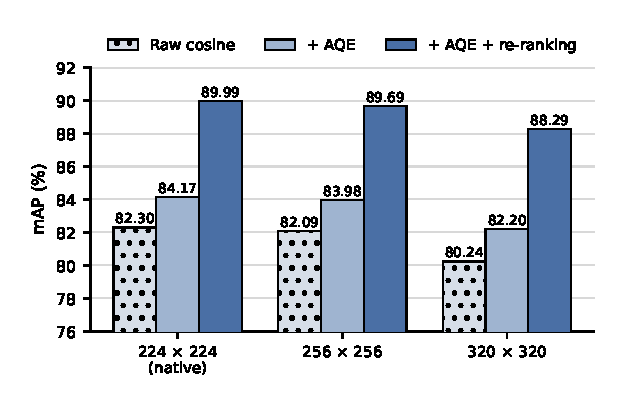
\includegraphics[width=0.88\columnwidth]{Fig9}
  \caption{Inference-resolution sensitivity of the deployed Stream~1
  checkpoint, which was trained at 224\,$\times$\,224. Position embeddings are
  bicubically interpolated at evaluation time and post-processing parameters
  are held identical. Accuracy degrades monotonically away from the native
  resolution at every stage of the pipeline}
  \label{fig:resolution}
\end{figure}
